\documentclass[a4paper,12pt, oneside]{book}

% \usepackage{fullpage}
\usepackage[italian]{babel}
\usepackage[utf8]{inputenc}
\usepackage{amssymb}
\usepackage{amsthm}
\usepackage{graphics}
\usepackage{amsfonts}
\usepackage{listings}
\usepackage{amsmath}
\usepackage{amstext}
\usepackage{engrec}
\usepackage{rotating}
\usepackage[safe,extra]{tipa}
%\usepackage{showkeys}
\usepackage{multirow}
\usepackage{hyperref}
\usepackage{mathtools}
\usepackage{microtype}
\usepackage{enumerate}
\usepackage{braket}
\usepackage{marginnote}
\usepackage{ulem}
\usepackage{bm}
\usepackage{pgfplots}
\usepackage{cancel}
\usepackage{polynom}
\usepackage{booktabs}
\usepackage{enumitem}
\usepackage{framed}
\usepackage{algorithm}
\usepackage{algpseudocode}
\usepackage{pdfpages}
\usepackage{pgfplots}
\usepackage[cache=false]{minted}

\usepackage[usenames,dvipsnames]{pstricks}
\usepackage{epsfig}
\usepackage{pst-grad} % For gradients
\usepackage{pst-plot} % For axes
\usepackage[space]{grffile} % For spaces in paths
\usepackage{etoolbox} % For spaces in paths
\makeatletter % For spaces in paths
\patchcmd\Gread@eps{\@inputcheck#1 }{\@inputcheck"#1"\relax}{}{}
\makeatother

\usepackage{tikz}\usetikzlibrary{er}\tikzset{multi
  attribute /.style={attribute ,double  distance =1.5pt}}\tikzset{derived
  attribute /.style={attribute ,dashed}}\tikzset{total /.style={double
    distance =1.5pt}}\tikzset{every  entity /.style={draw=orange ,
    fill=orange!20}}\tikzset{every  attribute /.style={draw=MediumPurple1,
    fill=MediumPurple1!20}}\tikzset{every
  relationship /.style={draw=Chartreuse2, fill=Chartreuse2!20}}
\newcommand{\key}[1]{\underline{#1}}

\usepackage{fancyhdr}
\pagestyle{fancy}
\fancyhead[LE,RO]{\slshape \rightmark}
\fancyhead[LO,RE]{\slshape \leftmark}
\fancyfoot[C]{\thepage}
\usepackage{tikz}
\usetikzlibrary{automata,positioning}


\title{Assignment 2, Bioinformatica}
\author{Davide Cozzi, 829827}
\date{}

\pgfplotsset{compat=1.13}
\begin{document}
\maketitle

\definecolor{shadecolor}{gray}{0.70}
\setlist{leftmargin = 2cm}
\newtheorem{teorema}{Teorema}
\newtheorem{definizione}{Definizione}
\newtheorem{esempio}{Esempio}
\newtheorem{corollario}{Corollario}
\newtheorem{lemma}{Lemma}
\newtheorem{osservazione}{Osservazione}
\newtheorem{nota}{Nota}
\newtheorem{esercizio}{Esercizio}

\renewcommand{\chaptermark}[1]{%
  \markboth{\chaptername
    \ \thechapter.\ #1}{}}
\renewcommand{\sectionmark}[1]{\markright{\thesection.\ #1}}
\tableofcontents
\chapter{Esercizio 1}
Per la specifica del problema abbiamo la seguente situazione:
\begin{itemize}
  \item \textbf{input}: una matrice di caratteri $M$ costruita su $\{0,1,*\}$,
  con al più due occorrenze di $*$. Si specifica che $M$ è una matrice
  $|S|\times |C|$, con ogni riga che rappresenta una specie dell'insieme $S$ e
  ogni colonna che rappresenta un carattere dell'insieme $C$ 
  \item \textbf{output}: un'eventuale matrice binaria di filogenesi perfetta
  $M_P$, anch'essa $|S|\times |C|$, o eventualmente un vettore di matrici
  binarie di filogenesi perfetta
\end{itemize}
Il ragionamento verte sulla presenza, all'interno della matrice $M$ in input,
eventualmente anche a priori rispetto alle possibili sostituzioni dei caratteri
$*$, della cosiddetta \textbf{matrice proibita}, che indico con $M_F$:
\[
  M_F=\left[
    \begin{matrix}
      1 & 0\\
      0 & 1\\
      1 & 1
    \end{matrix}
  \right]
\]
La presenza della matrice proibita infatti impedisce la costruzione di un albero
di filogenesi perfetta in quanto, con questa teoria, si ha un solo \textit{gain}
e nessun \textit{loss} per ogni carattere. In termini di albero di filogenesi
questa caratteristica si verifica avendo che ogni carattere etichetta un solo
ramo dell'albero e, una volta guadagnato un certo carattere, esso non verrà mai
perso. In altri termini, preso un nodo interno $w$ dell'albero di filogenesi, si
ha che tutti i caratteri, che etichettano i rami che dalla radice portano a quel
nodo, saranno presenti in tutte le foglie del sottoalbero che $w$ come
radice. Si ha quindi che un alberi di filogenesi perfetta esiste sse la matrice
da cui viene calcolato non contiene la matrice proibita in quanto dovrei avere
la ``perdita'' di uno dei due caratteri per poter rappresentare, in presenza
delle prime due specie, la terza, quella con entrambi i caratteri. \\
La verifica dell'assenza della matrice proibita può essere effettuata tramite il
controllo che la collezione delle colonne della matrice sia \textbf{laminare}.\\
Nel caso in esame però la matrice in input può contenere una o due posizioni
mancanti. Si ha che:
\begin{itemize}
  \item nel caso si abbia un solo $*$ esso può essere sostituito con o $0$ o $1$
  \item nel caso si abbiano due $*$ essi possono essere sostituiti,
  rispettivamente, da una delle seguenti coppie di valori binari:
  \[(0,0),(0,1),(1,0),(1,1)\]
\end{itemize}
Prima di effettuare le sostituzioni è possibile fare un controllo preliminare.
Si prenda la sottomatrice di $M$, che chiamiamo $M'$, composta da tutte le
colonne di $M$ in cui non si ha un simbolo $*$. Qualora $M'$ non abbia la
collezione di colonne laminare, avendo quindi all'interno la matrice proibita,
posso già concludere dicendo che non esiste alcuna sostituzione che permetta la
costruzione di una matrice di filogenesi perfetta. Questo controllo permette di
evitare diversi controlli di laminarità, di costo quadratico, in caso che la
matrice non ammetta filogenesi perfetta a priori rispetto alle sostituzioni. Il
controllo viene passato ``automaticamente'' qualora $M'$ sia di una sola
colonna. 
\begin{esempio}
  Vediamo un esempio di sottomatrice $M'$.
  Data:
  \[
    M=\left[
      \begin{matrix}
        1 & 0 & 0\\
        0 & * & 1\\
        1 & 0 & 1
      \end{matrix}
    \right]
  \]
  Si ottiene, rimuovendo la seconda colonna, la matrice:
  \[
    M'=\left[
      \begin{matrix}
        1 & 0\\
        0 & 1\\
        1 & 1
      \end{matrix}
    \right]
  \]
  che, in questo caso, non solo contiene la matrice proibita ma è la matrice
  proibita stessa. Quindi nessun valore di $*$ porterebbe ad una
  matrice di filogenesi perfetta.\\
  Come anticipato la verifica della presenza della matrice perfetta, a livello
  algoritmico, viene effettuata tramite il test di laminarità. Nel caso si
  analisi si produrrebbe la seguente matrice $L$:
  \[
    L=\left[
      \begin{matrix}
        -1 & 0\\
        0 & -1\\
        -1 & 1
      \end{matrix}
    \right]
  \]
  Dove si ha la seconda colonna con due valori non nulli diversi tra loro,
  avendo quindi che $M'$ non è laminare, contenendo la matrice proibita.
\end{esempio}
\noindent
Questo primo controllo è utile anche per calcolare l'esistenza della matrice di
filogenesi perfetta, e di conseguenza del relativo albero, qualora non si
abbiano correzioni da fare.\\
Passiamo ora ai casi in cui sia effettivamente possibile effettuare le
sostituzioni.\\
\textbf{Negli esempi successivi ho scelto di non mostrare ogni volta le matrici
  $L$ utili a verificare algoritmicamente la laminarità in quanto, avendo a che
  fare con toy examples, era facilmente individuabile la presenza della matrice
  proibita o meno. Il test viene comunque utilizzato nel piccolo codice usato
  come appoggio per questo esercizio.}
\section{Singola Sostituzione}
Avendo già verificato che la matrice, privata della singola colonna in cui è
presente il simbolo $*$, non contiene la matrice proibita non resta che
verificare se questo accade anche sostituendo con $0$ e con $1$. A priori
rispetto al resto della matrice in input non è verificabile se una
sostituzione sia valida o meno e, essendo il controllo tramite laminarità in
tempo $\mathcal{O}(|S|\cdot |C|)$ sulla matrice $M$ in input dopo aver
sostituito $*$, pare sensato procedere con entrambe le sostituzioni. A seconda
della matrice potrei ottenere una matrice di filogenesi solo sostituendo $*$ con
$1$ o solo con $0$ ma in determinati casi anche con entrambi.
\begin{esempio}
  Vediamo un esempio.\\
  Sia data in input la matrice (e si noti che la relativa matrice $M'$ non
  presenta all'interno la matrice proibita):
  \[
    M=\left[
      \begin{matrix}
        1 & 0 & 0\\
        1 & 1 & 0\\
        1 & * & 1
      \end{matrix}
    \right]\,\,\,\,\,\,\,\,\,\,\, M'=\left[
      \begin{matrix}
        1 & 0\\
        1 & 0\\
        1 & 1
      \end{matrix}
    \right]
  \]
  Si ha quindi una matrice con 3 specie, in ordine per riga $S1,S2,S3$, e 3
  caratteri, in ordine per colonna $C1,C2,C3$.\\
  Si hanno quindi le due matrici, sostituendo prima 0 e poi 1:
  \[M_0=\left[
      \begin{matrix}
        1 & 0 & 0\\
        1 & 1 & 0\\
        1 & 0 & 1
      \end{matrix}
    \right]\,\,\,\,\,\,\,\,\,\,\,M_1=\left[
      \begin{matrix}
        1 & 0 & 0\\
        1 & 1 & 0\\
        1 & 1 & 1
      \end{matrix}
    \right]
  \]
  In entrambi i casi è possibile effettuare con successo il test di linearità
  avendo quindi che in entrambi i casi è possibile costruire l'albero di
  filogenesi. Possiamo quindi chiamare tali matrici $M_{P_0}$ e $M_{P_1}$,
  avendo i rispettivi alberi di filogenesi perfetta:
  \begin{figure}[H]
    \centering
    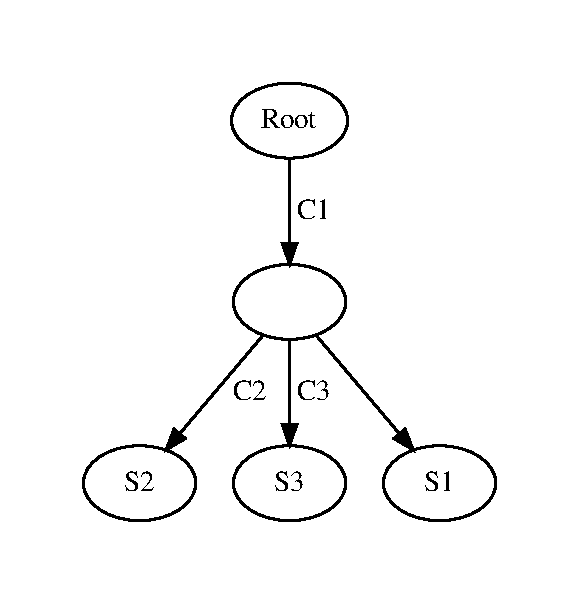
\includegraphics[scale = 0.5]{img/s1.pdf}
    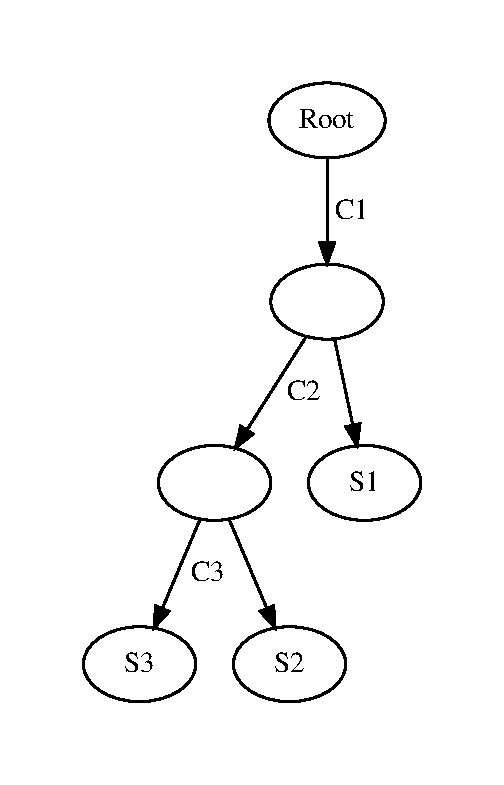
\includegraphics[scale = 0.5]{img/s2.pdf}
  \end{figure}
\end{esempio}
\section{Doppia Sostituzione}
Il caso con la doppia sostituzione è leggermente più complicato da trattare.\\
Come già anticipato, avendo due * nella matrice $M$ in input, posso avere 4
combinazioni possibili di correzioni:
\[(0,0),(0,1),(1,0),(1,1)\]
Si può quindi notare che in questo caso possiamo fare qualche ragionamento
aggiuntivo prima di effettuare il test di laminarità sull'intera matrice.\\
In questo caso infatti, qualora i due simboli $*$ non si trovino sulla stessa
colonna, è possibile effettuare un test di laminarità preliminare sulle due
colonne in cui sono presenti i $*$, ovviamente dopo aver effettuato la
sostituzione. Solo nel momento in cui questo primo test, di costo 
$\mathcal{O}(|S|\cdot 2)\approx\mathcal{O}(|S|)$, venga superato si procede al
più dispendioso test di laminarità sull'intera matrice, che ricordiamo essere di
costo $\mathcal{O}(|S|\cdot |C|)$. Vengono così limitati i test più
dispendiosi. \\ 
Anche in questo caso non pare possibile stabilire a priori quali sostituzioni
possano portare ad una matrice di filogenesi perfetta, senza passare per la
``batteria'' di test di laminarità sopra descritta.
\begin{esempio}
  Vediamo un esempio.\\
  Sia data in input la matrice $M$, il cui controllo di laminarità su $M'$,
  ottenuta da $M$ senza le colonne con i simboli $*$, non segnala
  problemi: 
  \[
    M=\left[
      \begin{matrix}
        1 & 0 & * & 0 & 0\\
        * & 1 & 1 & 0 & 1\\
        1 & 1 & 1 & 0 & 0\\
        0 & 0 & 0 & 1 & 0\\
      \end{matrix}
    \right]\,\,\,\,\,\,\,M'=\left[
      \begin{matrix}
        0 & 0 & 0\\
        1 & 0 & 1\\
        1 & 0 & 0\\
        0 & 1 & 0\\
      \end{matrix}
    \right]
  \]
  Si può quindi procedere con le varie sostituzioni, ricordando che, avendo i
  simboli $*$ su due colonne diverse, potremo effettuare i controlli di
  laminarità in primis sulla coppia di colonne con le sostituzioni.\\
  Si comincia con la coppia $(0,0)$, avendo quindi:
  \[
    M_{0,0}=\left[
      \begin{matrix}
        1 & 0 & \mathbf{0} & 0 & 0\\
        \mathbf{0} & 1 & 1 & 0 & 1\\
        1 & 1 & 1 & 0 & 0\\
        0 & 0 & 0 & 1 & 0\\
      \end{matrix}
    \right]
  \]
  Il primo test, quello di linearità sulla sottomatrice composta dalle due
  colonne con $*$, già segnala come si abbia la matrice proibita, infatti:
  \[
    M_{0,0}'=\left[
      \begin{matrix}
        1 & \mathbf{0} \\
        \mathbf{0} & 1\\
        1 & 1 \\
        0 & 0 \\
      \end{matrix}
    \right]
  \]
  Si può quindi concludere che la sostituzione $(0,0)$ non porterà ad una
  matrice di filogenesi perfetta.\\
  Si analizza quindi la seconda sostituzione, $(0,1)$:
  \[
    M_{0,1}=\left[
      \begin{matrix}
        1 & 0 & \mathbf{0} & 0 & 0\\
        \mathbf{1} & 1 & 1 & 0 & 1\\
        1 & 1 & 1 & 0 & 0\\
        0 & 0 & 0 & 1 & 0\\
      \end{matrix}
    \right]\,\,\,\,\,\,\,\,
    M_{0,1}'=\left[
      \begin{matrix}
        1 & \mathbf{0} \\
        \mathbf{1} & 1\\
        1 & 1 \\
        0 & 0 \\
      \end{matrix}
    \right]
  \]
  Dove si nota che né il primo controllo sulla sottomatrice né il test di
  laminarità sulla matrice 
  completa segnalano problemi quindi la matrice $M_{0,1}$ è una matrice di
  filogenesi perfetta, $M_{P_{0,1}}$.\\
  Si passa ad analizzare la terza sostituzione, $(1,0)$:
  \[
    M_{1,0}=\left[
      \begin{matrix}
        1 & 0 & \mathbf{1} & 0 & 0\\
        \mathbf{0} & 1 & 1 & 0 & 1\\
        1 & 1 & 1 & 0 & 0\\
        0 & 0 & 0 & 1 & 0\\
      \end{matrix}
    \right]\,\,\,\,\,\,\,\,
    M_{1,0}'=\left[
      \begin{matrix}
        1 & \mathbf{1} \\
        \mathbf{0} & 1\\
        1 & 1 \\
        0 & 0 \\
      \end{matrix}
    \right]
  \]
  In questo caso il primo test di linearità sulla sottomatrice non segnala
  problemi ma il test di linearità sulla matrice segnala come, a causa delle
  prime due colonne, la matrice $M_{1,0}$ non sia una matrice di filogenesi
  perfetta. \\
  Si arriva infine all'ultima correzione possibile, $(1,1)$:
  \[
    M_{1,1}=\left[
      \begin{matrix}
        1 & 0 & \mathbf{1} & 0 & 0\\
        \mathbf{1} & 1 & 1 & 0 & 1\\
        1 & 1 & 1 & 0 & 0\\
        0 & 0 & 0 & 1 & 0\\
      \end{matrix}
    \right]\,\,\,\,\,\,\,\,
    M_{1,1}'=\left[
      \begin{matrix}
        1 & \mathbf{1} \\
        \mathbf{1} & 1\\
        1 & 1 \\
        0 & 0 \\
      \end{matrix}
    \right]
  \]
  Anche in questo caso né il test di laminarità preliminare sulla sottomatrice
  né quello sulla matrice intera segnalano problemi, avendo infatti che
  $M_{1,1}$ è una matrice di filogenesi perfetta, $M_{P_{1,1}}$.\\
  Si ha quindi che sia la sostituzione $(0,1)$ che la sostituzione $(1,1)$
  portano ad avere due matrice di filogenesi perfetta, $M_{P_{0,1}}$ e
  $M_{P_{1,1}}$, coi rispettivi alberi: 
  \begin{figure}[H]
    \centering
    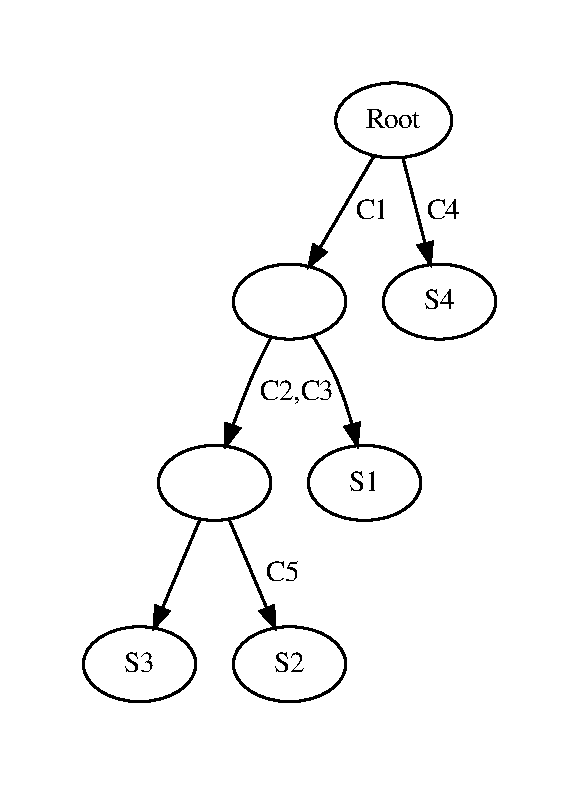
\includegraphics[scale = 0.5]{img/d1.pdf}
    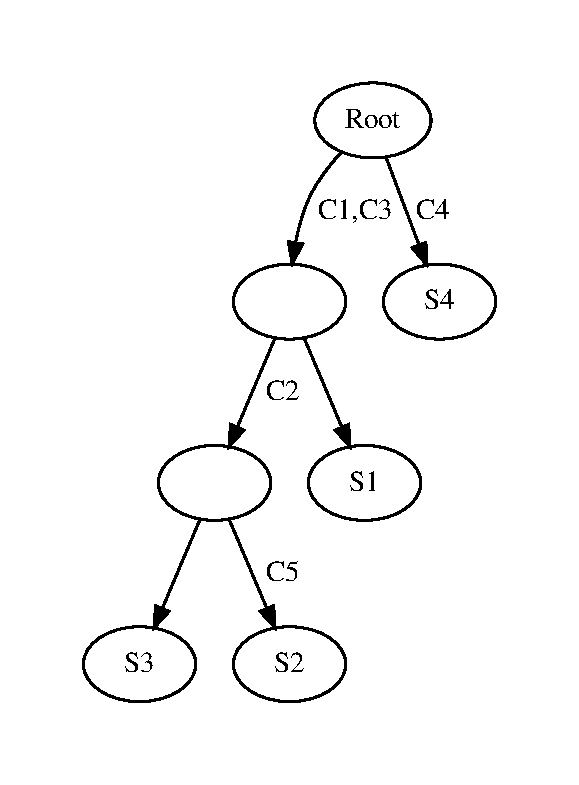
\includegraphics[scale = 0.5]{img/d2.pdf}
  \end{figure}
\end{esempio}
\section{Note Conclusive}
Come si è notato non sembra essere possibile prevedere le sostituzioni corrette,
in entrambi i casi, prima di effettuarle e verificarle, possibilmente con
controlli di laminarità su sottomatrici. L'unico caso per cui si può evitare di
procedere è quello in cui la matrice in input $M$ includa la matrice proibita
a priori rispetto alle sostituzioni.
Una volta ottenuta la singola matrice di filogenesi perfetta si segnala che
l'albero di filogenesi perfetta relativo è \textbf{unico}. In questo contesto
con ``unico'' si intende 
che dal nodo radice ad ogni foglia avrò sempre e comunque lo stesso insieme di
etichette per gli archi. Si segnala comunque che diverse sostituzioni possono
portare a diverse matrici valide e quindi altrettanti alberi (come visto negli
esempi).\\ 
Vediamo quindi una bozza di pseudocodice che codifica la procedura seguita. Si
hanno in primis i due pseudocodici relativi ai due tipi di sostituzione:
\begin{algorithm}[H]
  \small
  \begin{algorithmic}[1]
    \Function{OneCorrection}{$M$}
    \State $perfectPhylogenyVec\gets[\,\,\,]$
    \State $corrections \gets [0,1]$
    \For {$corr$ \textbf{in} $corrections$}
    \State $M_{corr}\gets correctWith(M, corr)$
    \If {$isLaminar(M_{corr})$}
    \State $push(perfectPhylogenyVec, M_{corr})$
    \EndIf
    \EndFor
    \State \textbf{return} $perfectPhylogenyVec$
    \EndFunction
  \end{algorithmic}
  \caption{Procedura per la correzione di un singolo errore}
\end{algorithm}
\begin{algorithm}[H]
  \small
  \begin{algorithmic}[1]
    \Function{TwoCorrection}{$M$}
    \State $perfectPhylogenyVec\gets[\,\,\,]$
    \State $corrections \gets [(0,0), (0,1), (1,0), (1,1)]$
    \For {$corr$ \textbf{in} $corrections$}
    \State $M_{corr}\gets correctWith(M, corr)$
    \State $M'_{corr}\gets columnsCorrectedWith(M, corr)$
    \If{$isLaminar(M_{corr}')\land isLaminar(M_{corr})$}
    \State $push(perfectPhylogenyVec, M_{corr})$
    \EndIf
    \EndFor
    \State \textbf{return} $perfectPhylogenyVec$
    \EndFunction
  \end{algorithmic}
  \caption{Procedura per la correzione di un doppio errore}
\end{algorithm}
Nel secondo caso, quello con la doppia sostituzione, si noti come l'operazione
di \textit{and} all'interno dell'\textit{if} verifichi in primis la laminarità
delle colonne, qualora siano due (avendo che il controllo di laminarità su
singola colonna è automaticamente passato), su cui sono state effettuate le
correzioni.
\newpage
\noindent
Si ha quindi lo pseudocodice con l'unione delle due possibili categorie di
correzione, in presenza di singolo errore o doppio, che calcola le varie
possibili matrici di filogenesi perfetta e restituisce un array contenente esse
e il conto dei possibili alberi:
\begin{algorithm}[H]
  \small
  \begin{algorithmic}[1]
    \Function{CheckPerfect}{$M$}
    \State $errCount \gets countError(M)$
    \State $M'\gets subMatrixNoError(M)$
    \If{$\neg isLaminar(M')$}
    \State \textbf{return} $\emptyset$
    \EndIf
    \State $perfectPhylogenyVec\gets[\,\,\,]$
    \If{$errCount == 0$}
    \State \textbf{return} $[perfectPhylogeny(M)]$
    \ElsIf{$errCount == 1$}
    \State $perfectPhylogenyVec\gets OneCorrection(M)$
    \Else
    \State $perfectPhylogenyVec\gets TwoCorrection(M)$
    \EndIf
    \State $treeCount \gets length(perfectPhylogenyVec)$
    \State \textbf{return} $(perfectPhylogenyVec,\,treeCount)$
    \EndFunction
  \end{algorithmic}
  \caption{Procedura per la verifica di filogenesi perfetta con al più
  due sostituzioni}
\end{algorithm}

\chapter{Esercizio 2}
Per il problema in analisi si ha:
\begin{itemize}
  \item \textbf{input}: una matrice $M_G$, $n\times m$, di $n$ genotipi
  costruita su $\{0,1,*,?\}$, dove $0/1$ rappresentano i rispettivi siti
  omozigoti, $*$ rappresenta i siti eterozigoti e $?$ rappresenta i dati
  mancanti 
  \item \textbf{output}: una matrice $M_H$, $2\cdot n\times m$, di aplotipi,
  costruita 
  su $\{0,1\}$ tale che ogni genotipo dello matrice in input $M_G$ sia risolto
  da una coppia di aplotipi della matrice $M_H$ e che $M_H$ sia matrice di
  filogenesi perfetta
\end{itemize}
\begin{definizione}
  Si ha che la coppia di aplotipi $\langle h_1,h_2\rangle$, visti come
  vettori su alfabeto $\{0,1\}$, \textbf{risolve} il
  genotipo $g$, visto come vettore su alfabeto $\{0,1,*\}$, sse, $\forall i$:
  \[
    \begin{cases}
      h_1[i]\neq h_2[i]&\mbox{se } g[i]=*\\
      g[i]=h_1[i]=h_2[i]&\mbox{altrimenti}
    \end{cases}
  \]
\end{definizione}
\begin{definizione}
  La matrice di aplotipi $M_H$ \textbf{risolve} la matrice di genotipi $M_G$
  sse:
  \[\forall g\in M_G,\,\,\,\exists h_1,h_2\in
    M_H\mbox{ t.c. }\langle h_1,h_2\rangle \mbox{ risolve } g\]
\end{definizione}
La strategia per risolvere la matrice di genotipi con la matrice di aplotipi
consiste quindi, in primis, nell'effettuare le possibili correzioni. Qualora si
corregga un dato mancante con un sito omozigote 0 o 1 si ha che in fase di
costruzione della matrice degli aplotipi verranno costruite due righe con 0 o 1,
rispettivamente, in quella precisa posizione. Qualora il dato venga invece
corretto tramite un sito eterozigote si avrà, nella matrice di aplotipi, una
coppia di righe con due valori complementari per quella posizione.\\
Si intuisce quindi come la complessità del problema cresca in primis
all'aumentare dei dati mancanti nella matrice $M_G$, aumentando le possibili
combinazioni di 0, 1 e * per poter correggere la matrice prima di poter
effettivamente tentare di risolverla con una matrice di aplotipi. Inoltre, in
fase di risoluzione con la matrice di aplotipi, un'elevata presenza di siti
eterozigoti nel medesimo genotipo, quindi nella stessa riga, comporta che si
abbiano potenzialmente molte matrici di aplotipi da controllare, per trovare
quella che effettivamente risolve la matrice di genotipi e ammette anche
filogenesi perfetta. \\
Una possibile strategia di ottimizzazione del problema potrebbe essere quella di
avere una sorta di \textit{reference}, tramite il quale escludere, in prima
battuta, alcune strategie di correzione dei dati mancanti e, in seconda battuta,
poter velocizzare la scelta di coppie di aplotipi che risolvano un genotipo con
vari siti eterozigoti.
\section{Conclusioni ed Esempio}
Come si è descritto il problema non sembra prevedere una soluzione ``facile''.\\
Si propone quindi un piccolo toy example con un solo dato mancante.
\begin{esempio}
  Sia data la matrice:
  \[
    M_G= \left[
      \begin{matrix}
        * & ? \\
        1 & 1 \\
        0 & 1 
      \end{matrix}
    \right]
  \]
  Le possibili correzioni sono le seguenti:
  \[
    M_{G_0}= \left[
      \begin{matrix}
        * & \mathbf{0} \\
        1 & 1 \\
        0 & 1 
      \end{matrix}
    \right]M_{G_1}= \left[
      \begin{matrix}
        * & \mathbf{1} \\
        1 & 1 \\
        0 & 1 
      \end{matrix}
    \right]M_{G_*}= \left[
      \begin{matrix}
        * & \bm{*} \\
        1 & 1 \\
        0 & 1 
      \end{matrix}
    \right]
  \]
  Dopo aver effettuato le correzioni bisogna costruire le possibili matrici di
  aplotipi, secondo le regole sopra definite.\\
  Iniziamo con $M_{G_0}$:
  \[M_{G_0}'
    = \left[
      \begin{matrix}
        1 & 0 \\
        0 & 0 \\
        1 & 1 \\
        1 & 1 \\
        0 & 1 \\
        0 & 1 
      \end{matrix}
    \right]
  \]
  Dove si nota la matrice proibita quindi sicuramente la sostituzione con il
  sito omozigote 0 non è una sostituzione accettabile.\\ 
  Passiamo a $M_{G_1}$:
  \[M_{G_1}'
    = \left[
      \begin{matrix}
        1 & 1 \\
        0 & 1 \\
        1 & 1 \\
        1 & 1 \\
        0 & 1 \\
        0 & 1 
      \end{matrix}
    \right]
  \]
  Che si nota non contenere la matrice proibita quindi la sostituzione con il
  sito omozigote 1 sarebbe una sostituzione accettabile. Si ottiene quindi una
  matrice di aplotipi valida, che, essendo ottenuta sostituendo 1, chiamiamo
  $M_{H_1}$.\\ 
  Si ha infine $M_{G_*}$ che, a causa del doppio sito eterozigote nello stesso
  genotipo comporta due possibili matrici di aplotipi:
  \[M_{G_*}'    = \left[
      \begin{matrix}
        1 & 1 \\
        0 & 0 \\
        1 & 1 \\
        1 & 1 \\
        0 & 1 \\
        0 & 1 
      \end{matrix}
    \right]
    M_{G_*}''
    = \left[
      \begin{matrix}
        1 & 0 \\
        0 & 1 \\
        1 & 1 \\
        1 & 1 \\
        0 & 1 \\
        0 & 1 
      \end{matrix}
    \right]
  \]
  Notando che solo $M_{G_*}'$ ammette effettivamente filogenesi perfetta quindi
  la sostituzione del dato mancante con un sito eterozigote $*$ non sempre porta
  ad una matrice di aplotipi di filogenesi perfetta. $M_{G_*}''$ infatti
  contiene la matrice proibita. Chiamo tale 
  matrice di aplotipi valida, essendo ottenuta sostituendo $*$, $M_{H_*}$.
\end{esempio}
Si è visto quindi come il problema della ricostruzione di matrici di aplotipi a
partire da una matrice di genotipi con errori sembri essere un problema
complesso, a causa, in primis, della moltitudine di correzioni possibili e, in
seconda battuta, a causa della procedura di calcolo di valide matrici di
aplotipi a partire da una matrice di genotipi senza dati mancanti.
\chapter{Codice per la Filogenesi Perfetta}
Si segnala che nei primi due esercizi è stato usato come appoggio il seguente
codice: \url{https://github.com/dlcgold/perfect-phylogeny-rs}.\\
Questo piccolo tool in Rust contiene i due algoritmi visti a lezione per la
verifica della laminarità e la creazione dell'albero di filogenesi. È anche
presente una bozza di correzioni secondo la procedura indicata per il primo
esercizio.\\ 
Per quanto il codice fosse solo abbozzato è stato comodo per la creazione degli
alberi di filogenesi perfetta del primo esercizio e per alcuni test durante lo
svolgimento del secondo e quindi mi è sembrato giusto segnalarlo. 
\chapter{Esercizio 3}
Per questo problema si hanno:
\begin{itemize}
  \item \textbf{input}: una \textit{matrice di $n$ frammenti di aplotipi}
  $M$, per la quale sono eventualmente ammessi indel e spazi. La matrice
  quindi è costruita su $\{0,1,-\}$ e, essendo costruita su $m$ SNPs, è di
  dimensioni $n\times m$. Tale matrice è assunta poter non essere
  \textit{error-free}   
  \item \textbf{output}: una bipartizione delle righe di $M$ in due insiemi di
  frammenti, $H_1$ e $H_2$, tali che, all'interno del singolo insieme, non si
  abbiano \textit{conflitti}. Tali insiemi rappresentano quindi due aplotipi,
  avendo quindi che il conflitto tra frammenti avviene solo tra due aplotipi
  differenti. Tale bipartizioni potrebbe non esistere
\end{itemize}
\begin{definizione}
  Preso un insieme di frammenti di aplotipi $F=\{f_1,f_2,\ldots, f_n\}$ si ha
  che $f'\in F$ e $f''\in F$ sono in \textbf{conflitto} sse $f'\in H_1$ e
  $f''\in H_2$, ovvero sse:
  \[\exists i \in [1,m]\mbox{ t.c. }f'[i]\neq f''[i]\mbox{ con } f'[i]\neq
    \mbox{"-"}\land f''[i]\neq \mbox{"-"}\]
  Quindi se prese due righe esiste almeno una posizione (su indice di colonna in
  pratica) in cui non si ha lo stesso valore su entrambe. Si noti come spazi e
  indel, indicati sempre con 
  ``-'', vengono ``ignorati'' in quanto rappresentano una mancanza di
  informazione e possiamo quindi ``immaginarli'' come un valore
  desiderato. Questo ultimo aspetto si applica in tutte le situazioni 
  dell'esercizio in cui si specifica che i ``-'' vengono ignorati.
\end{definizione}
Avendo assunto che la matrice potrebbe non essere \textit{error-free} bisogna
procedere con la correzione degli stessi, tramite, ad esempio, l'algoritmo
k-cMEC. Tale algoritmo risolve il problema di ottimo di trovare il minimo numero
di correzioni per l'intera matrice di frammenti, con al più $k$ correzioni per
colonna, necessarie per ottenere una matrice che ammette bipartizione.\\
Da specifica, inoltre, si ha che il numero massimo di correzioni per colonna è
uno, quindi si ha, per l'algoritmo k-cMEC, $k=1$. Nel dettaglio con il termine
\textit{correzione} si intende l'operazione di \textit{flip} di un valore, da 0
a 1 o viceversa, trascurando quindi gli indel e gli spazi, per gli stessi motivi
espressi sopra.\\
Da specifica, in aggiunta, si assume che la matrice $M$ in input è priva di gap
interni.\\ 
Si ha quindi, per l'algoritmo di correzione:
\begin{itemize}
  \item \textbf{input}: una matrice $M$ di $n$ frammenti di aplotipi non
  \textit{error-free}, come definita sopra
  \item \textbf{output}: una matrice $M'$, qualora esista, di dimensioni uguali
  a $M$, anch'essa costruita su $\{0,1,-\}$, \textit{error-free}, costruita a
  partire da $M$ con al più una singola correzione per colonna
\end{itemize}
Prima di dare un'idea dell'algoritmo bisogna dare qualche definizione.
\begin{definizione}
  Una colonna $j$ di una matrice $M$ di $n$ frammenti di aplotipi è detta
  \textbf{omozigote} sse:
  \[\forall i\in[1,n],\,\,\, M_j[i]=0\lor M_j[i]=\mbox{"-"}\]
  oppure sse:
  \[\forall i\in[1,n],\,\,\, M_j[i]=1\lor M_j[i]=\mbox{"-"}\]
  In altri termini se la colonna, al più degli indel e degli spazi, è formata o
  da soli zeri o da soli uni.\\
  Una colonna priva di questa caratteristica, avendo quindi valori diversi oltre
  a quello di indel e spazi, è detta \textbf{eterozigote}.
\end{definizione}
\begin{definizione}
  Prese due colonne, $j'$ e $j''$ di una matrice $M$ di $n$ frammenti di
  aplotipi si ha che esse sono dette \textbf{colonne concordanti} se vale una
  delle seguenti condizioni:
  \begin{itemize}
    \item entrambe le colonne sono omozigote
    \item entrambe le colonne sono eterozigote e si ha che, a parità di indice,
    tutti i valori della prima colonna sono il complementare dei valori della
    seconda
    \item una colonna è omozigote e l'altra eterozigote
  \end{itemize}
  Per la seconda condizione (anche se implicitamente questo discorso, come visto
  nella definizione precedente, si applica anche agli altri due casi) si
  trascurano indel e spazi, quindi la condizione vale:
  \[\forall i\in[1,n] \mbox{ t.c } M_{j'}[i]\neq \mbox{"-"}\land M_{j''}[i]\neq 
    \mbox{"-"}\]
  Tutti e tre i casi permettono quindi la bipartizione delle righe della coppia
  di colonne.
\end{definizione}
\noindent
Si noti che una colonna omozigote non presenta particolari informazioni in
merito alla questione della bipartizione, avendo tutti valori uguali.
\begin{teorema}
  Si può dimostrare che si può ottenere una bipartizione da una matrice $M$
  di $n$ frammenti di aplotipi senza gap interni sse ogni coppia di
  colonne concorda.
\end{teorema}
\noindent
Si propone quindi un'idea di base per l'ottenimento della matrice $M'$,
\textit{error free}, a partire da $M$, con al più una correzione per colonna.\\
L'idea di base è che si procede scorrendo da sinistra a destra le colonne di
$M$, correggendo la colonna $j$ basandosi eventualmente sulle prime $j-1$
colonne, con eventuali branch per le possibili correzioni.\\
La correzione della colonna $j$, qualora venga effettivamente fatta, può
comportare la costruzione di una colonna omozigote o di una colonna
eterozigote. In questo secondo caso la colonna $j$ deve essere concordante con
almeno un'altra colonna tra $1$ e $j-1$.\\
Per tenere traccia del minimo numero di correzioni fino alla colonna $j$ si usa
$D(1,j)$ e diciamo che esso viene calcolato a partire da $D(1,j-1)$, qualora
possibile. Il limite di una sola correzione per colonna infatti potrebbe
comportare il non ottenimento della matrice $M'$ e per indicare il fatto in
termini matematici diciamo che in tal caso si ha:
\[D(1,j)=\infty\]
Chiamiamo $d(j',j'')$ una funzione equivalente alla distanza di Hamming,
adattata a conteggiare le differenze tra colonne due colonne, $j'$ e $j''$.\\
Definiamo quindi una funzione che calcola il numero di correzioni sulla colonna
$j''$ necessarie per renderla concorde con la colonna $j$:
\[c(j',j'')=
  \begin{cases}
    0&\mbox{se } d(j',j'')=0\\
    1&\mbox{se } d(j',j'')=1 \land j'\mbox{ concorde } j''\\
    \infty&\mbox{altrimenti}
  \end{cases}
\]
Possiamo quindi definire una bozza di equazione di ricorrenza per il calcolo del
minimo numero di correzioni necessarie ad ottenere $M'$, con il vincolo di avere
al più una correzione per colonna:
\[D(1,j)=\min_{j\in[2,n]}
  \begin{cases}
    D(1,j-1)+\min
    \begin{cases}
      c(\vec{0},j)\\
      c(\vec{1},j)
    \end{cases}
    \mbox{, con $j$ omozigote}\\
    D(1,j-1)+\min_{i\in[1,j-1]}c(i,j)\mbox{, con $i,j$ eterozigote}
  \end{cases}
\]
Avendo quindi il minimo tra due casi, in ordine:
\begin{itemize}
  \item il caso omozigote, che viene calcolato sommando a $D(1,j-1)$ il minimo
  numero, che potrebbe essere 0, 1 o $\infty$, di flip atti a ottenere una
  matrice omozigote
  \item il caso eterozigote, che viene calcolato sommando a $D(1,j-1)$ il minimo
  numero, che potrebbe essere 0, 1 o $\infty$, di flip atti a ottenere una
  colonna eterozigote concordante con una delle prime $|j-1|$ colonne. Qualora
  non esista una colonna $i\in [1,j-1]$ eterozigote si assume $c(i,j)=0$ (in
  quanto una colonna omozigote ed una eterozigote concordano e quindi non sono
  necessarie correzioni)
\end{itemize}
Ovviamente se entrambi i casi restituiscono che il minimo di flip è $\infty$ si
conclude che non è possibile ottenere una matrice $M'$ \textit{error free} che
ammetta bipartizione. Eventuali colonne di soli ``-'' vengono ignorate.\\
In base a quanto detto possiamo dire che vale la \textit{sottostruttura
  ottima}. Questo è dovuto al fatto che di procede
partendo da $D(1,j-1)$, che quindi viene assunto ottimo, per il calcolo di
$D(1,j)$, che o lascia uguale $D(1,j-1)$ o lo incrementa di uno (l'incremento di
$\infty$ invece segnalerebbe l'impossibilità di avere un ottimo).\\

\textit{Si noti che che l'algoritmo tiene conto delle ipotetiche correzioni,
  tenendo appunto conto del minor numero di correzioni con al più un flip per
  colonna, senza però effettuarle veramente, limitandosi a calcolare il numero
  minimo di correzioni. È comunque una bozza è non ho dimostrazioni tangibili
  del fatto che effettivamente funzioni ma sembra essere comunque un punto di
  partenza accettabile. D'altro canto la ricostruzione effettiva della matrice
  $M'$ è un problema non banale che deve tenere conto di più branch possibili di
  correzione e non viene analizzato in questo assignment.}\\

\noindent
Una volta ottenuta la matrice $M'$ di $n$ frammenti di aplotipi
\textit{error-free} possiamo ridurre il problema della ricerca della
bipartizione in un problema sui grafi:
\begin{itemize}
  \item \textbf{input}: una matrice $M'$ di $n$ frammenti di aplotipi
  \textit{error-free} che si è visto ammettere bipartizione. Si chiami
  $F=\{f_1,f_2,\ldots, f_n\}$ l'insieme delle righe, ovvero l'insieme degli $n$
  frammenti 
  \item \textbf{output}: un grafo bipartito, non orientato, indicato con $G
  =(V,E)$ e detto \textbf{grafo dei conflitti}, dal quale si estraggono le due
  partizioni, ovvero $H_1$ e $H_2$
\end{itemize}
\newpage
La costruzione di tale grafo è la seguente:
\begin{itemize}
  \item l'insieme dei nodi del grafo è formato dall'insieme dei frammenti,
  ovvero $V=F$
  \item l'insieme degli archi del grafo è formato dagli archi che collegano
  frammenti di $F$ in conflitto, ovvero, presi due nodi $f'$ e $f''$ (che
  ricordiamo rappresentano anche due frammenti):
  \[(f',f'')\in E \iff \mbox{$f'$ in conflitto con $f''$}\]
\end{itemize}
Una volta costruito il grafo si hanno algoritmi polinomiali per la verifica
della bipartizione e per l'identificazione della stessa. Si ottengono quindi,
qualora esistano, i due aplotipi $H_1$ e $H_2$.\\

\noindent
Ricapitolando l'intero problema:
\begin{enumerate}
  \item \textbf{input}: una matrice $M$ di $n$ frammenti di aplotipi,
  eventualmente non \textit{error-free}, come già definita
  \item si effettua, se possibile, la correzione di $M$ in $M'$ tramite
  \textit{1-cMEC} 
  \item si costruisce l'eventuale grafo dei conflitti $G=(V,E)$, a partire da
  $M'$, come definito sopra. Si noti che, qualora il grafo esista, esso ammette
  bipartizione in quanto costruito ottenuto da una matrice \textit{error-free}
  che ammette bipartizione
  \item \textbf{output:} l'eventuale bipartizione nei due aplotipi $H_1$ e
  $H_2$, calcolata a partire da $G$. Qualora la matrice non possa essere
  corretta con 1-cMEC sicuramente non si avrà bipartizione per le ipotesi fatte
  e quindi l'algoritmo segnalerà l'errore
\end{enumerate}
\textit{Come discusso a lezione, si potrebbe ragionare anche in ottica di grafo
  dei conflitti per poter procedere con la correzione degli
  errori. Ipoteticamente, una volta costruito il grafo $G=(V,E)$ a partire dalla
  matrice non \textnormal{error-free} in input, qualora non
  ammetta bipartizione, si potrebbe procedere con un algoritmo che elimina
  determinati archi al fine di ottenere una bipartizione. Tale soluzione non
  viene però qui approfondita ma una prima analisi sembra portare a pensare che
  anche questa soluzione sia, almeno in parte, esponenziale.} 
\end{document}
% LocalWords:  sottostringhe sottostringa pseudocodice lowercase Hamming
% LocalWords:  sottoalbero sottomatrice sottomatrici pseudocodici
% LocalWords:  algoritmicamente
